\documentclass[landscape]{article}
\usepackage{lmodern}
\usepackage{amssymb,amsmath}
\usepackage{ifxetex,ifluatex}
\usepackage{fixltx2e} % provides \textsubscript
\ifnum 0\ifxetex 1\fi\ifluatex 1\fi=0 % if pdftex
  \usepackage[T1]{fontenc}
  \usepackage[utf8]{inputenc}
\else % if luatex or xelatex
  \ifxetex
    \usepackage{mathspec}
  \else
    \usepackage{fontspec}
  \fi
  \defaultfontfeatures{Ligatures=TeX,Scale=MatchLowercase}
\fi
% use upquote if available, for straight quotes in verbatim environments
\IfFileExists{upquote.sty}{\usepackage{upquote}}{}
% use microtype if available
\IfFileExists{microtype.sty}{%
\usepackage{microtype}
\UseMicrotypeSet[protrusion]{basicmath} % disable protrusion for tt fonts
}{}
\usepackage[margin=1in]{geometry}
\usepackage{hyperref}
\hypersetup{unicode=true,
            pdftitle={CS 765 Rough Sketches},
            pdfauthor={Brad Stieber},
            pdfborder={0 0 0},
            breaklinks=true}
\urlstyle{same}  % don't use monospace font for urls
\usepackage{color}
\usepackage{fancyvrb}
\newcommand{\VerbBar}{|}
\newcommand{\VERB}{\Verb[commandchars=\\\{\}]}
\DefineVerbatimEnvironment{Highlighting}{Verbatim}{commandchars=\\\{\}}
% Add ',fontsize=\small' for more characters per line
\usepackage{framed}
\definecolor{shadecolor}{RGB}{248,248,248}
\newenvironment{Shaded}{\begin{snugshade}}{\end{snugshade}}
\newcommand{\KeywordTok}[1]{\textcolor[rgb]{0.13,0.29,0.53}{\textbf{{#1}}}}
\newcommand{\DataTypeTok}[1]{\textcolor[rgb]{0.13,0.29,0.53}{{#1}}}
\newcommand{\DecValTok}[1]{\textcolor[rgb]{0.00,0.00,0.81}{{#1}}}
\newcommand{\BaseNTok}[1]{\textcolor[rgb]{0.00,0.00,0.81}{{#1}}}
\newcommand{\FloatTok}[1]{\textcolor[rgb]{0.00,0.00,0.81}{{#1}}}
\newcommand{\ConstantTok}[1]{\textcolor[rgb]{0.00,0.00,0.00}{{#1}}}
\newcommand{\CharTok}[1]{\textcolor[rgb]{0.31,0.60,0.02}{{#1}}}
\newcommand{\SpecialCharTok}[1]{\textcolor[rgb]{0.00,0.00,0.00}{{#1}}}
\newcommand{\StringTok}[1]{\textcolor[rgb]{0.31,0.60,0.02}{{#1}}}
\newcommand{\VerbatimStringTok}[1]{\textcolor[rgb]{0.31,0.60,0.02}{{#1}}}
\newcommand{\SpecialStringTok}[1]{\textcolor[rgb]{0.31,0.60,0.02}{{#1}}}
\newcommand{\ImportTok}[1]{{#1}}
\newcommand{\CommentTok}[1]{\textcolor[rgb]{0.56,0.35,0.01}{\textit{{#1}}}}
\newcommand{\DocumentationTok}[1]{\textcolor[rgb]{0.56,0.35,0.01}{\textbf{\textit{{#1}}}}}
\newcommand{\AnnotationTok}[1]{\textcolor[rgb]{0.56,0.35,0.01}{\textbf{\textit{{#1}}}}}
\newcommand{\CommentVarTok}[1]{\textcolor[rgb]{0.56,0.35,0.01}{\textbf{\textit{{#1}}}}}
\newcommand{\OtherTok}[1]{\textcolor[rgb]{0.56,0.35,0.01}{{#1}}}
\newcommand{\FunctionTok}[1]{\textcolor[rgb]{0.00,0.00,0.00}{{#1}}}
\newcommand{\VariableTok}[1]{\textcolor[rgb]{0.00,0.00,0.00}{{#1}}}
\newcommand{\ControlFlowTok}[1]{\textcolor[rgb]{0.13,0.29,0.53}{\textbf{{#1}}}}
\newcommand{\OperatorTok}[1]{\textcolor[rgb]{0.81,0.36,0.00}{\textbf{{#1}}}}
\newcommand{\BuiltInTok}[1]{{#1}}
\newcommand{\ExtensionTok}[1]{{#1}}
\newcommand{\PreprocessorTok}[1]{\textcolor[rgb]{0.56,0.35,0.01}{\textit{{#1}}}}
\newcommand{\AttributeTok}[1]{\textcolor[rgb]{0.77,0.63,0.00}{{#1}}}
\newcommand{\RegionMarkerTok}[1]{{#1}}
\newcommand{\InformationTok}[1]{\textcolor[rgb]{0.56,0.35,0.01}{\textbf{\textit{{#1}}}}}
\newcommand{\WarningTok}[1]{\textcolor[rgb]{0.56,0.35,0.01}{\textbf{\textit{{#1}}}}}
\newcommand{\AlertTok}[1]{\textcolor[rgb]{0.94,0.16,0.16}{{#1}}}
\newcommand{\ErrorTok}[1]{\textcolor[rgb]{0.64,0.00,0.00}{\textbf{{#1}}}}
\newcommand{\NormalTok}[1]{{#1}}
\usepackage{graphicx,grffile}
\makeatletter
\def\maxwidth{\ifdim\Gin@nat@width>\linewidth\linewidth\else\Gin@nat@width\fi}
\def\maxheight{\ifdim\Gin@nat@height>\textheight\textheight\else\Gin@nat@height\fi}
\makeatother
% Scale images if necessary, so that they will not overflow the page
% margins by default, and it is still possible to overwrite the defaults
% using explicit options in \includegraphics[width, height, ...]{}
\setkeys{Gin}{width=\maxwidth,height=\maxheight,keepaspectratio}
\IfFileExists{parskip.sty}{%
\usepackage{parskip}
}{% else
\setlength{\parindent}{0pt}
\setlength{\parskip}{6pt plus 2pt minus 1pt}
}
\setlength{\emergencystretch}{3em}  % prevent overfull lines
\providecommand{\tightlist}{%
  \setlength{\itemsep}{0pt}\setlength{\parskip}{0pt}}
\setcounter{secnumdepth}{0}
% Redefines (sub)paragraphs to behave more like sections
\ifx\paragraph\undefined\else
\let\oldparagraph\paragraph
\renewcommand{\paragraph}[1]{\oldparagraph{#1}\mbox{}}
\fi
\ifx\subparagraph\undefined\else
\let\oldsubparagraph\subparagraph
\renewcommand{\subparagraph}[1]{\oldsubparagraph{#1}\mbox{}}
\fi

%%% Use protect on footnotes to avoid problems with footnotes in titles
\let\rmarkdownfootnote\footnote%
\def\footnote{\protect\rmarkdownfootnote}

%%% Change title format to be more compact
\usepackage{titling}

% Create subtitle command for use in maketitle
\newcommand{\subtitle}[1]{
  \posttitle{
    \begin{center}\large#1\end{center}
    }
}

\setlength{\droptitle}{-2em}
  \title{CS 765 Rough Sketches}
  \pretitle{\vspace{\droptitle}\centering\huge}
  \posttitle{\par}
  \author{Brad Stieber}
  \preauthor{\centering\large\emph}
  \postauthor{\par}
  \date{}
  \predate{}\postdate{}


\begin{document}
\maketitle

\section{\texorpdfstring{\pagenumbering{gobble}}{}}\label{section}

\newpage 

\begin{center}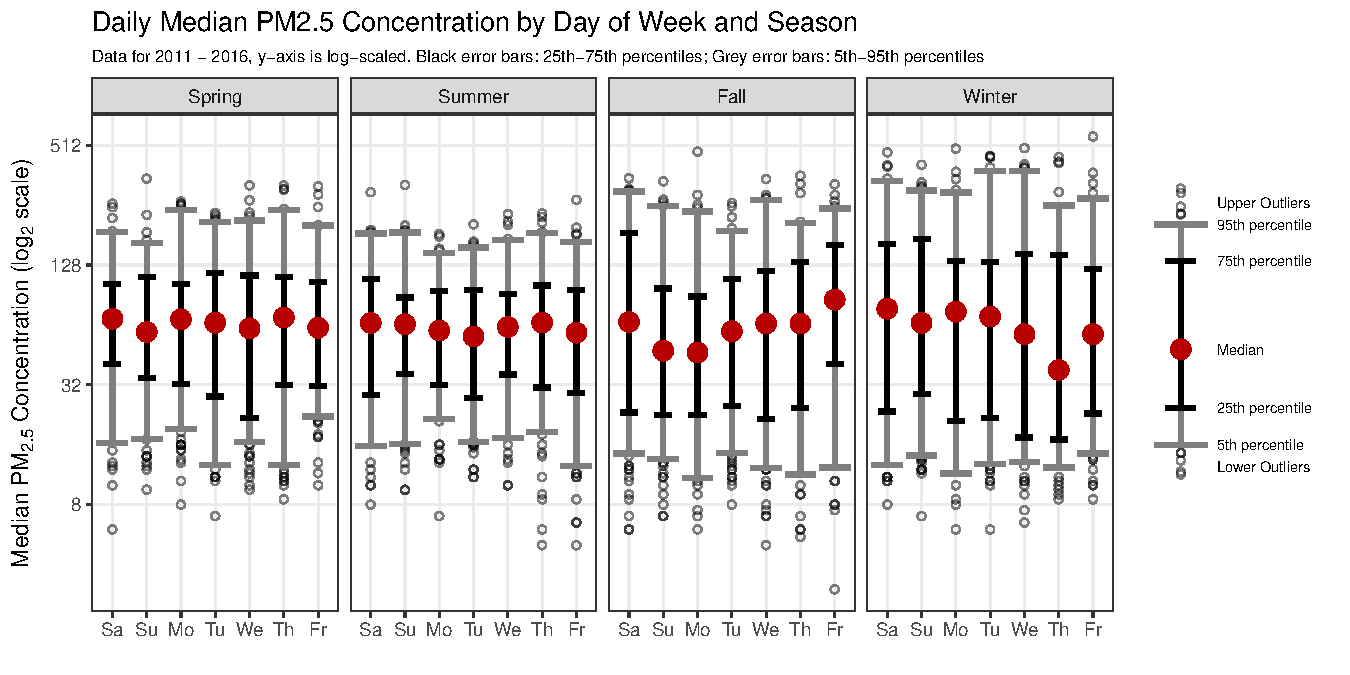
\includegraphics{RoughSketches_files/figure-latex/unnamed-chunk-2-1} \end{center}

\textbf{Data} Daily median pollution levels (higher indicates more
pollution) for 2011 - 2016 by day of week and season

Plot of daily median \(PM_{2.5}\) concentration levels (measure of
pollution) by day of week and season. \textbf{Red dots are the overall
medians, black error bars represent 25 - 75th percentile range, and grey
error bars represent 5 - 95th percentile range.} Outlier points are
those that fall above or below the 5 - 95th percentile range. The y-axis
is \(log_2\) scaled.

We were originally trying to compare pollution levels by weekday /
weekend. We were interested in investigating whether pollution levels
were elevated during the work week. Instead, we found that although the
levels remain fairly flat between seasons and day of week, the variation
in pollution levels tends to increase in the Fall and Winter. Note that
the error bars tend to be longer in the Fall and Winter than those in
the Spring or Summer. The lengthening of error bars indicates
differences in seasonal variability.

\newpage

\begin{center}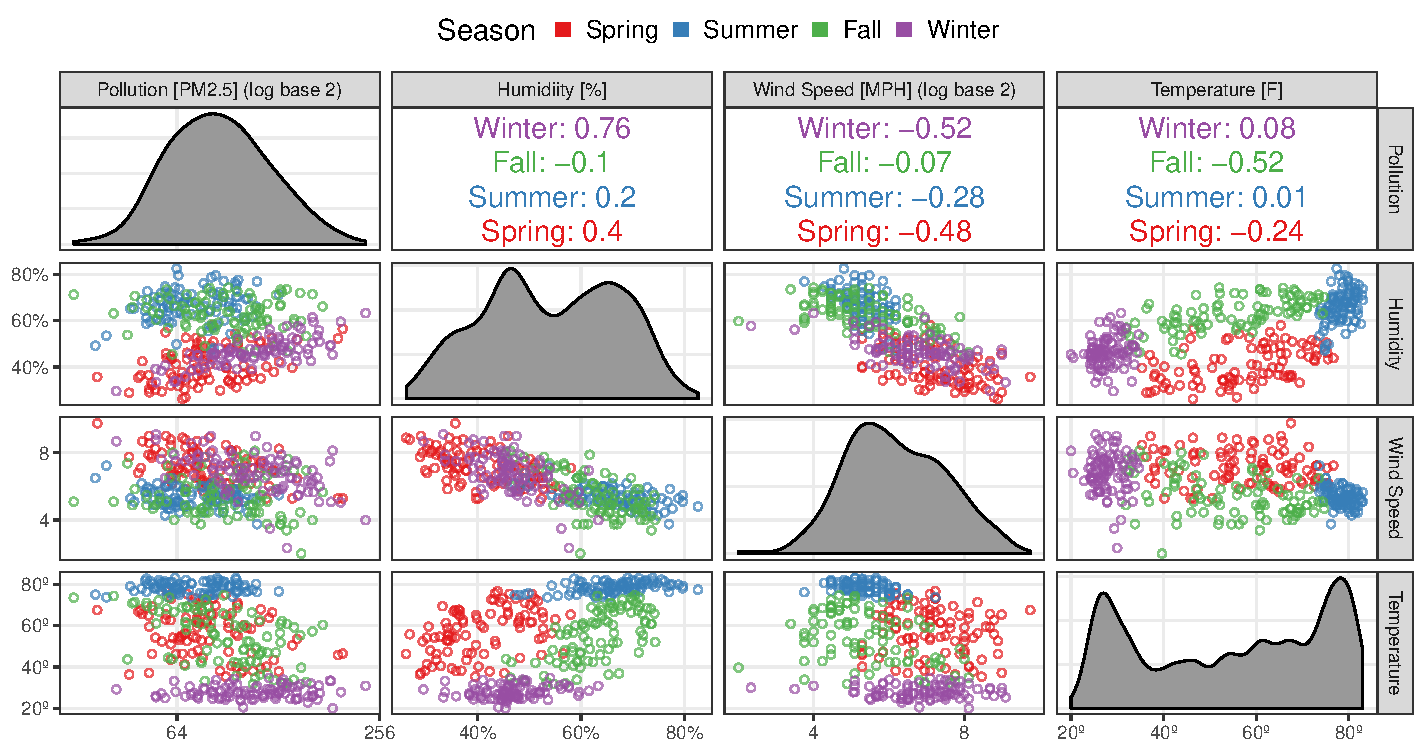
\includegraphics{RoughSketches_files/figure-latex/unnamed-chunk-3-1} \end{center}

\textbf{Data} Average of the daily averages for pollution (higher values
indicate more pollution), humidity, wind speed, and temperature for 2011
- 2016.

What relationships exist between pollution, humidity, wind speed, and
temperature? Do these relationships vary depending on season? What do
the distributions of these values look like? This visualization allows
for many distinct queries into the complex relationships between season
and our quantitative metrics.

We display a scatter plot matrix investigating pollution, humidity, wind
speed, and temperature. Points are colored according to the season. Each
value displayed is the average of the 2011-2016 daily averages. We
choose a relatively high level of aggregation to avoid over-plotting.
There should be approximately 365 marks on each scatter plot. We also
display the correlations for each season between \(log_2\) pollution and
humidity, \(log_2\) wind speed, and temperature. The axes for pollution
and wind speed are \(log_2\) scaled.

\newpage

\textbf{Alternative Encoding of SPLOM}

\begin{center}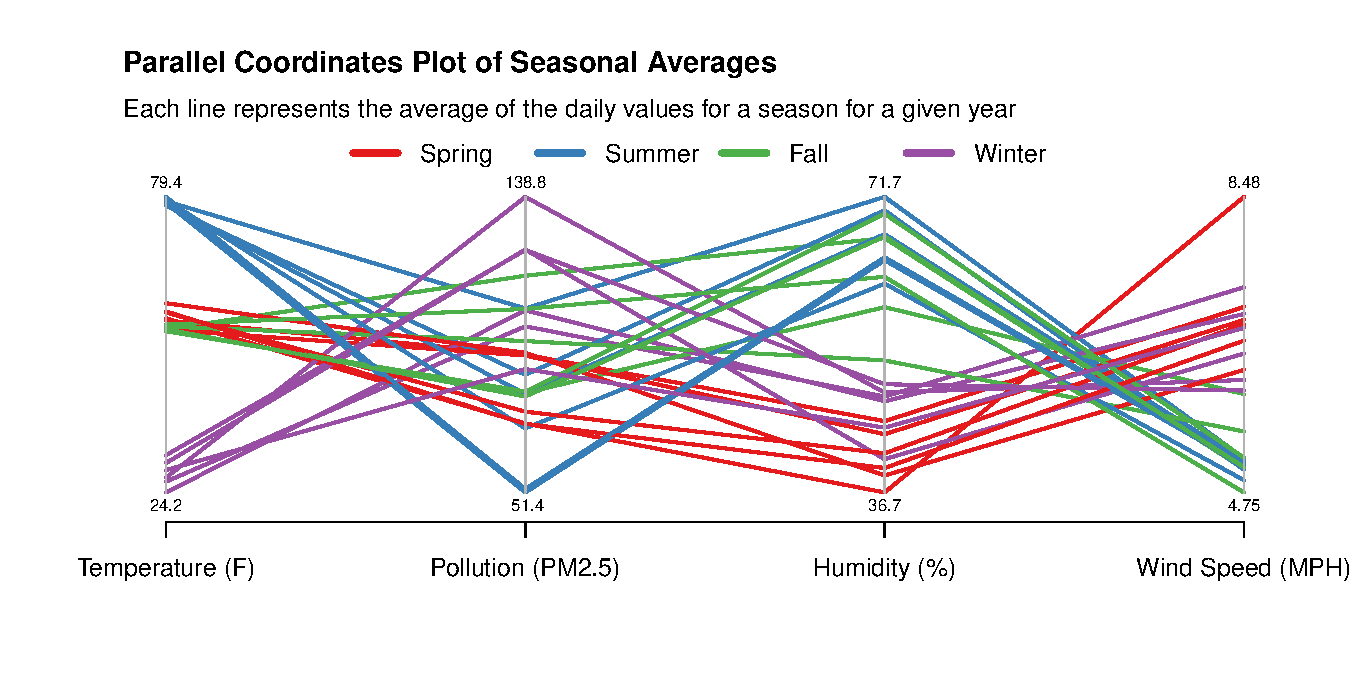
\includegraphics{RoughSketches_files/figure-latex/unnamed-chunk-4-1} \end{center}

\textbf{Data} Averages of daily averages for pollution (higher values
indicate more pollution), humidity, wind speed, and temperature for 2011
- 2016, by year and season.

What relationships exist between pollution, humidity, wind speed, and
temperature? Do these relationships vary depending on season? What do
the distributions of these values look like?

Parallel coordinates plot investigating pollution, humidity, wind speed,
and temperature. Lines are colored according to the season. Each line
represents the average of the daily values for each season for each
year. Though less dense than the scatter plot matrix, we are still able
to ascertain some of the relationships between our quantitative metrics.

\newpage

\begin{center}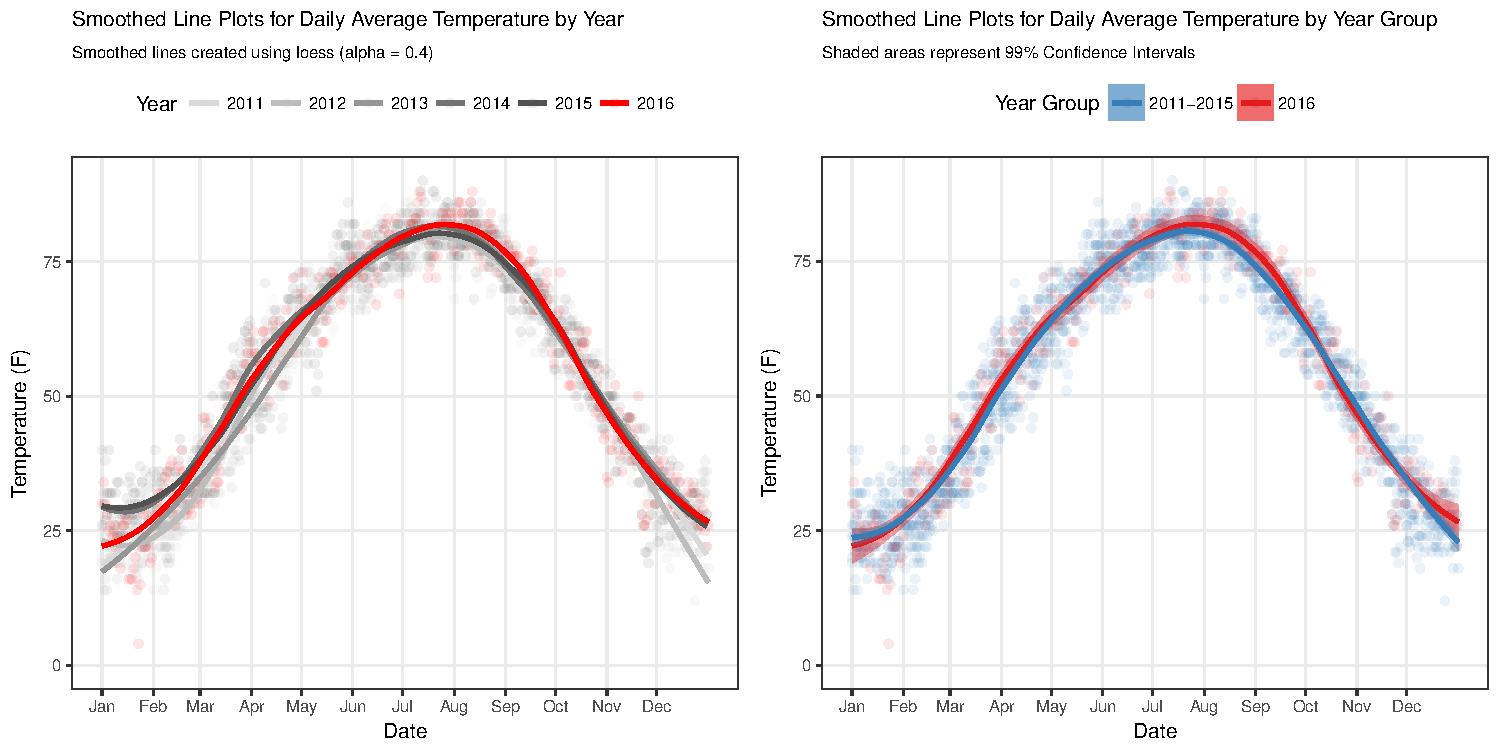
\includegraphics{RoughSketches_files/figure-latex/unnamed-chunk-5-1} \end{center}

\textbf{Data} Daily average temperatures for 2011 - 2016 by day of year

Climate change is a major concern for many people. Even though our time
frame is too short to make any clear scientific judgments, we
investigate the temperature trends for 2016 versus previous years to
look for signs of warming. We choose to emphasize the smoothed curves
rather than the actual data to avoid spurious observations from
variability in the daily data.

We display a two panel graph which utilizes a \texttt{loess} fitting
method to smooth out the variability in daily average temperature data.
Our left panel compares the smoothed trend for the previous years
(varying shades of gray) to the smoothed trend from 2016 (red line). We
color the 2016 line red to make it pop-out in the display. The right
panel compares the smoothed trend for a model fit on 2011-2015 data
versus a model fit on the 2016 data. The prediction from the smoothed
trend for 2016 was higher than the year group trend on 241 (66\%) days.
In the left panel, we display the predictions with no confidence
intervals, in the right panel we display the predictions as well as 99\%
confidence intervals.

\begin{Shaded}
\begin{Highlighting}[]
\KeywordTok{power.prop.test}\NormalTok{(}\DataTypeTok{p1 =} \FloatTok{0.001}\NormalTok{, }\DataTypeTok{p2 =} \FloatTok{0.0011}\NormalTok{, }
                \DataTypeTok{sig.level =} \NormalTok{.}\DecValTok{05}\NormalTok{, }\DataTypeTok{power =} \NormalTok{.}\DecValTok{95}\NormalTok{, }\DataTypeTok{alternative =} \StringTok{'one.sided'}\NormalTok{)}
\end{Highlighting}
\end{Shaded}

\begin{verbatim}
## 
##      Two-sample comparison of proportions power calculation 
## 
##               n = 2270268
##              p1 = 0.001
##              p2 = 0.0011
##       sig.level = 0.05
##           power = 0.95
##     alternative = one.sided
## 
## NOTE: n is number in *each* group
\end{verbatim}


\end{document}
